\section{Schur Decomposition}
\label{sec:nonreversible}

%projections/clusterings
All previous projections of processes onto metastable sets were based on the assumption of \textbf{reversibility}.
%All previous decompositions of state spaces into metastable sets were based on the assumption of a \textbf{reversible} process.
%unfortunately, reversibility is not fulfilled for many real-world processes
Unfortunately, many real-world processes are \textbf{not} reversible. In that case the corresponding transfer operator is not self-adjoint and therefore we have to deal with possibly complex eigenvalues and eigenfunctions/eigenvectors, which is not compatible with PCCA+. %\ref{thm:selfadjoint_reversible}
%If we want to compute a metastable decomposition for a nonreversible process, we have to face the problem of possibly complex eigenvalues and eigenfunctions/eigenvectors.
%In that case we cannot apply PCCA+.
%\marginpar{real eigvec needed?}
%that the eigenvalues/eigenvectors might be complex valued and thus, PCCA+ is not applicable. \marginpar{of transf.op.?}
This problem can be circumvented by considering the real Schur decomposition of the transition matrix instead of its spectral decomposition. 
%One possibility/alternative/way to circumvent this problem is to consider the real Schur decomposition of the transition matrix instead of its spectral decomposition.
This yields an invariant subspace of real Schur vectors on which we can apply PCCA+.
%enables us to, allowing us
%Then, we can apply PCCA+ to the real Schur vectors of the matrix instead to its eigenvectors.
%possible, feasible
This approach is feasible, since the real Schur vectors span the same subspace as the corresponding complex Schur vectors and those span the same subspace as the corresponding eigenvectors. \marginpar{see ...}

\marginpar{?}%Besides/Beyond/In addition/Additionally. enabling/allowing us
Beyond enabling us to analyze non-reversible processes, this new approach yields several more advantages, like allowing us to identify a broader class of structures, including dominant cycles or sinks.
%and being independent of a positive stat. distribution?


\subsubsection*{NESS processes}

The method we present in this section is only employable for finite processes.
%In this section, we present a method which is employable only for finite processes. 
Therefore we consider in the following an irreducible and aperiodic (i.e. ergodic) Markov chain on the finite state space $E = \{1,\dots,N\}$ given by the transition matrix $P$. By irreducibility and aperiodicity, the process possesses a unique invariant measure $\pi$ being positive everywhere. %\marginpar{stat. dist.} \marginpar{see ..}
Then $\pi$ is the normalized eigenvector of $P$ for the unique eigenvalue $\lambda_1 = 1$. \marginpar{$\mu$?}

%We begin with introducing a certain class of processes that are nonreversible, but still have some nice properties.

\begin{defi}[NESS process]
A Markov process is called \textit{nonequilibrium steady state (NESS)} process if it is nonreversible, but still has a steady state, given by an invariant measure $\pi$, such that the process is ergodic with respect to $\pi$.
% ergodic wrt pi -> converges against pi?
\end{defi}

%\begin{equation*}
%p_\tau(A,B) = p(\tau,A,B) =  \Prob(X_\tau = B \mid X_0 = A)
%\end{equation*}
As a NESS process is nonreversible, there are regions where the detailed balance equation is not fulfilled, i.e. there is an effective probability flow $p(\tau, A, B) - p(\tau,B,A) \neq 0$ between some subsets $A,B \subset E$ of the state space.

\begin{defi}[Flow Matrix]
The probability flow associated to a Markov process is given by the flow matrix
\begin{equation*}
F = DP,
\end{equation*}
where $P$ is the transition matrix of the process and $D$ the diagonal matrix $D = \diag (\pi_1, \dots, \pi_N)$ with the entries of the invariant measure $\pi$.
\end{defi}
So the (steady state) probability flow from state $i$ to $j$ is given by $F_{ij} = \mu_i P_{ij}$.
If the process is reversible, the flow matrix $F$ is symmetric due to detailed balance. For a NESS process, $F$ is not symmetric since there are states $i,j \in E$ with $F_{ij} \neq F_{ji}$.
\newpage

%dominant cycles have similar properties as dominant sets for reversible processes, i.e. large eigenvalues with $|\lambda| \approx 1$. But now the eigenvalues are lying in the %complex plane and might be non-real (pairs of complex eigenv.).

%What is a metastable cycle?
%\begin{defi}[Dominant Cycle]
%= metastable cycle?
%\end{defi}
%a cycle is dominant if there is a high probability inside the Markov chain to follow this cycle.

%What is the dominant structure of a nonreversible process? ibland cycle, ibland set?
%What is the problem with nonreversible processes? non-real eigenvalues

%invariant sets?
%Dominant structures will be defined utilizing the dominant Schur vectors of the transition matrix instead of its eigenvectors.
%A membership matrix can be defined as a linear combination of these leading Schur vectors (spectral clustering with PCCA+).

%\subsubsection*{Spectrum of a NESS process}

\subsubsection*{Schur Decomposition} %Schur values vs eigenvalues

We have the same objective as in the previous section: given a Markov process acting on a large state space $E$, a projection onto a smaller state space $\{1,\dots,n\}$ is aimed at, where each cluster represents one metastable set of the process.
%We have the same aim as in the previous sections: we are given a Markov process acting on a large state space $E$ and want to project it onto a smaller state space $\{1,\dots,n\}$, where each cluster represents one metastable set of the process.
For this purpose, we introduce a matrix decomposition generalizing the spectral decomposition. %extending, generalizing

\begin{defi}[Schur Decomposition]
Let $P \in \mathbb{R}^{N \times N}$ be a transition matrix. Then it can be written as
\begin{equation}
\label{eq:def_schur}
X\inv PX = \Lambda,
\end{equation}
where $X$ is a unitary matrix and $\Lambda$ is an upper triangular matrix, having $\lambda_1, \dots, \lambda_N$ as diagonal entries, which is called a \textit{Schur decomposition} of $P$.
If $X = [v_1 \mid \cdots \mid v_N]$ is a column partitioning of $X$, then the $v_i$ are referred to as \textit{Schur vectors}.
\end{defi}

The existence of such a matrix $X$ is shown in Golub and van Loan\cite[Theorem 7.1.3]{golub1996}.
Since $\Lambda$ is similar to $P$, both matrices have the same eigenvalues.   %spectrum, $\sigma(P) = \sigma(\Lambda)$.
Since $\Lambda$ is triangular, they correspond to the diagonal entries $\lambda_1, \dots, \lambda_N$ of $\Lambda$.
The Schur vectors $v_k$ satisfy
\begin{equation*}
	Pv_k = \lambda_k v_k + \sum_{i=1}^{k-1} n_{ik} v_i, \ \ k=1,\dots,N,
\end{equation*}
and therefore span an invariant subspace given by
\begin{equation*}
S_k = \mathrm{span}\{v_1,\dots,v_k\}.
\end{equation*}
Moreover, if we choose a matrix $X_k = [v_1 \mid \dots \mid v_k]$, then $\sigma(X_k\inv P X_k) = \{\lambda_1, \dots, \lambda_k\}$.
%A Schur decomposition is not unique.?
The eigenvalues $\lambda_i$ in \eqref{eq:def_schur} can be arbitrarily ordered by an appropriate choice of $X$.
%permuting the columns of $X$.
Thus each subset of $k$ eigenvalues induces at least one $k$-dimensional invariant subspace.
%Restriction on some Schur vectors useful later when we just want to consider dominant Schur vectors
\\

%employed
For our purpose, decomposition \eqref{eq:def_schur} is not sufficient, since it can include complex Schur vectors.
As $P$ is a real matrix, its non-real eigenvalues come in complex conjugate pairs. This fact can be utilized to build a \textit{real Schur decomposition}, where both $X$ and $\Lambda$ are real matrices.
%As we are interested in \textbf{real} Schur vectors, we take advantage of the real Schur decomposition.
Though this alternative decomposition does not yield a triangular matrix, but only a \textit{quasi-triangular} one, allowing $2 \times 2$-blocks on its diagonal. %result/yield
%\marginpar{picture}

\begin{thm}[Real Schur Decomposition]
%Röblitz p. 22
If $P \in \R^{N \times N}$, then there exists an orthogonal matrix $X_s \in \R^{N \times N}$ such that
\begin{equation*}
X_s\inv PX_s = \Lambda_s,
\end{equation*}
where $\Lambda_s$ is block-triangular with $1 \times 1$ and $2 \times 2$-blocks on its diagonal. The $1 \times 1$-blocks contain the real eigenvalues of $P$ and the eigenvalues of the $2 \times 2$-blocks are the complex eigenvalues of $P$.
\end{thm}
A proof can be found in Golub and van Loan\cite[Theorem 7.4.1]{golub1996}.
%Since the matrix $X_s$ is orthogonal, we have $X_s^T = X_s^{-1}$.
Each real matrix can be decomposed into such an upper quasi-triangular matrix. Thus the real Schur decomposition can be considered as an ``eigenvalue-revealing'' decomposition; %interpreted
the real and the imaginary part of the complex eigenvalues are easily obtained from the $2 \times 2$-blocks.

%\subsubsection*{Cases of nonreversible processes}
%\subsubsection*{Different types of nonreversible processes}
%\subsubsection*{Meaning of the block-diagonal structure}
\subsubsection*{Block-diagonal structure}

%employ, make use of. take advantage of
We want to make use of the real Schur decomposition to analyze transition matrices.
Depending on the shape of the quasi-triangular matrix $\Lambda_s$, we can not only find out informations about the eigenvalues of $P$, but also on the reversibility of the corresponding process.
% we can classify different kinds of nonreversible processes.
A case study is presented in Weber\cite{Weber2017} and shortly summarized in the following.
%Different cases are described in
\\

%determined/measured
%Originally& by its definition
By definition, the reversibility of a process is determined by the flow matrix $F = DP$. According to detailed balance, a process is reversible if and only if this matrix is symmetric.
%Hence it is nonreversible if this matrix is not symmetric.
%However, there are different kinds of nonsymmetry of that matrix possible, which will be described now.
However, nonreversibility of $P$ can as well be identified by its Schur decomposition $\Lambda_s$. %identified/related/revealed/connected
%finf out/see


A Schur decomposition is block-diagonal with eigenvalues and $2 \times 2$-blocks on its diagonal. The meaning of an $1 \times 1$-block as an eigenvalue is clear, so we are just going to analyze the shape of such an $2 \times 2$-block and its influence on reversibility and eigenvalues of $P$.
%the matrix $\Lambda_s$ will always be of the following shape:
Assume we are given the Schur decomposition
\begin{equation}
\label{eq:schur_block}
\Lambda_s = 
\begin{tikzpicture}[baseline=-0.5ex]
\matrix [matrix of math nodes,left delimiter=(,right delimiter=)] (m)
{
	1    & 0  & 0     \\
	0 & \lambda_2   & \epsilon      \\
	0   & -\delta    & \lambda_3       \\
} ;

\draw (m-2-2.north west) rectangle (m-3-3.south east);
\end{tikzpicture}
\end{equation}
with $\epsilon,\delta \geq 0$.
We examine the properties of this matrix (eigenvalues, reversibility) by inserting different values for $\epsilon$ and $\delta$ in the $2 \times 2$-block.

%caused/related/connected
%As nonreversibility of the process is caused by the non-symmetry of that matrix, and hence by the existence of $2 \times 2$-blocks, we have to analyze such a block.
%We will see that the location of nonsymmetric entries and the multiplicity of eigenvalues play a role for that.

%The type of nonreversibility depends on the multiplicity of eigenvalues and on the location of nonsymmetric entries.

%Measure degree of nonreversibility by this matrix? ||DQ-Q^TD|| bzw. dyadisches Produkt der Schur-Vektoren..


\begin{description}
	\item [Reversible] If $\epsilon = \delta = 0$ and furthermore $\lambda_2 \neq \lambda_3$, then $\Lambda_s$ is a diagonal matrix and $P$ is reversible.
	In this case, the eigenvalues are identical to the Schur values, $\Lambda_e = \Lambda_s$, and the eigenvectors are identical to the Schur vectors, $X_e = X_s$.
	
	%Shape: diagonal matrix (always?) = Eigendecomposition
	%no double eigenvalues? or double eigenvalues with geom = alg vielfachheit possible?
	
	Reversibility of $P$ is equivalent to the symmetry of $\Lambda_s$ (+ geometric and algebraic multiplicities should correspond; no double eigenvalues).
	\item [Nonreversible with real eigenvalues] If we add an additional upper diagonal element $\epsilon > 0$, then we make $\Lambda_s$ asymmetric.
	The eigenvalues of $P$ correspond to the entries $\lfam$ on the diagonal of $\Lambda_s$.
	The eigenvectors of $P$ are real, but \textbf{not $\pi$-orthogonal} anymore. In contrast to that, the Schur decomposition still leads to $\pi$-orthogonal Schur vectors $X_s$.
	
	Non-reversibility of $P$ can be seen by the fact that the Schur matrix $\Lambda_s$ is not symmetric. \marginpar{?}
	
	%Shape: upper diagonal element $\epsilon$.
	
	%Problem: corresponding eigenvectors are not D-orthogonal anymore. \marginpar{but at least real}
	
	%But: Schur vectors (real) are still orthogonal. by trick eigenvalues can be made orthogonal?
	\item[Nonreversible and not diagonalizable] If $\lambda_2 = \lambda_3$ with $\epsilon > 0$ and $\delta = 0$, then $P$ has an ``incomplete'' $2 \times 2$-block, meaning that it has an eigenvalue whose geometrical multiplicity does not correspond to its algebraic multiplicity.
	Therefore, $P$ does not have an eigendecomposition and is not diagonalizable. 
	
	Since $P$ is not diagonalizable, it is non-reversible.
	
	While the eigendecomposition does \textbf{not exist}, the Schur decomposition still exists.
	%and yields pi-orthogonal Schur vectors
	
	%A reversible matrix is always diagonalizable. Thus if we find a matrix which is not diagonalizable (for instance by eigenvalues with different algebraic and geometric multiplicities), then we %instantly know that it has to be nonreversible.
	
	%Thus a non-diagonalizable matrix has no Eigendecomposition. Hence it is useful to apply the Schur decomposition, because it always exists.
	\item[Nonreversible with complex eigenvalues] If $\lambda_2 = \lambda_3$ and additionally $\epsilon, \gamma > 0$, then we have a ``complete'' $2 \times 2$-block, encoding the existence of two \textbf{complex eigenvalues}.
	
	The complex-valued spectrum implies the non-reversibility of $P$.
	%(and existence of complex eigenvectors)
	However, the Schur decomposition still yields \textbf{real} Schur vectors.
	
	%Shape: complete $2 \times 2$-block.
	
	%Problem: complex eigenvectors. Good: Schur vectors are real.
	
	%\subsubsection*{Ordering Eigenvalues in the Real Schur Form \cite[Theorem 7.6.2]{golub1996}}
	%p. 396
\end{description}

%occur/appear/arise
Summarized, there are several problems that can appear when dealing with the {eigen-decomposition} of non-reversible processes.
The existence of an eigendecomposition is not always given (not diagonalizable matrix).
Moreover it can happen that the eigenvectors are not $\pi$-orthogonal or contain complex entries, which is problematic for the use of PCCA+.
However, we can circumvent these issues by using the real Schur vectors instead.
%However, all of that can be circumvented by using the real Schur decomposition instead,
%since it always exists and provides real and $\pi$-orthogonal Schur vectors.
%Good premises for applying PCCA+!


%\subsubsection*{GenPCCA: Clustering wrt metastable sets}
\subsubsection*{GenPCCA: Clustering in terms of Schur vectors}

%We have the same aim as in section \ref{sec:fuzzy}. Again,...
The aim is to cluster a given process $P$ into metastable sets based on membership functions $\chi = XA$.
%However, we have seen that eigenvectors of non-reversible processes are problematic
%in order that the computed solution
%the algorithm/ the application. compute/return/produce/yield. not the case/not achieved. meaningful projection/solution
However, the application of PCCA+ requires certain conditions to be fulfilled in order to yield a meaningful projection, which is in general not the case for eigenvectors of a non-reversible process.
%However we have seen that inserting eigenvectors of a nonreversible process into PCCA+ does not result in a meaningful solution
%As PCCA+ using eigenvectors is not applicable for nonreversible processes, we present an approach involving Schur vectors.
%including nonreversible processes
%For the eigenvectors of a non-reversible process 
A solution replacing them by Schur vectors has been proposed by Fackeldey and Weber\cite{fackeldey2017gen}. Their approach is a generalization of PCCA+ and therefore called Gen-PCCA (``Generalized-Perron Cluster Cluster Analysis'').

%In order to execute a suitable projection, we analyze at first the conditions 

%correct/suitable. analyze/identify. necessary/sufficient?
Looking back to the proof of theorem \ref{thm:iteration_error}, we identify two conditions implying a correct projection, i.e. a projection without discretization error.
%or Markovian? G(P^k) = (G(P))^k
%\ref{thm:iteration_error} ensures us a correct projection under membership functions $\chi = XA$.
The matrix $X \in \R^{N \times n}$ has to span an invariant subspace by
%fulfill the invariant subspace condition %span an invariant subspace
\begin{equation}
\label{eq:invariant}
PX = X\Lambda
\end{equation}
for $\Lambda \in \R^{n \times n}$. Furthermore, the orthogonality relation \marginpar{why $\eta$ enough?}
\begin{equation}
\label{eq:orthogonal}
X^T D_\eta X = I,
\end{equation}
has to be satisfied with respect to some initial distribution $\eta$.
%invariant subspace condition always fulfilled for eigenvectors, as it is the definition of eigenvectors?
\\

%As we can see from a comparison with the previous case study, these two properties are not fulfilled for the eigendecomposition of a non-reversible process.
These properties are in general not fulfilled for the eigendecomposition of a nonreversible process, as we can see from a comparison with the previous case study. For a non-reversible process, the eigenvectors can be complex or non-orthogonal. Moreover, it is not even guaranteed that $P$ is diagonalizable. \marginpar{  trick} %not even
%The eigenvectors of a nonreversible process having real eigenvalues are \textbf{not} orthogonal (because of non-symmetry of $DP$ or $\Lambda_s$?). 
\\

%constructed/chosen
However, real Schur vectors for a stochastic matrix $P$ can always be constructed such that they satisfy both criteria. In order to do so, the following symmetrization trick can be applied. If $\xtilde$ are $n$ Schur vectors of $\widetilde{P} = D^{0.5} P D^{-0.5}$, then we get \marginpar{same for eigen}%obtain 
\begin{equation*}
\begin{aligned}
& \   & & \widetilde{P} \xtilde = \xtilde \Lambda  \\
\Leftrightarrow & \ & & D^{0.5} P D^{-0.5} \xtilde = \xtilde \Lambda \\
\Leftrightarrow & \ & & P D^{-0.5} \xtilde =  D^{-0.5} \xtilde \Lambda \\
\Leftrightarrow & \ & & P X = X \Lambda, \textrm{ with } X = D^{-0.5} \xtilde.
\end{aligned}
\end{equation*}
%then by some easy calculations, we get the Schur vectors $X = D^{-0.5} \xtilde$ corresponding to $PX = X \Lambda$.
Since Schur vectors of a symmetric matrix are always orthogonal, the same holds for its multiplication with a diagonal matrix.
Thus, we are guaranteed that $X$ fulfill conditions \eqref{eq:invariant} and \eqref{eq:orthogonal}.
A further advantage in comparison to the previous section is, that by this trick, orthogonality can be achieved for \textbf{any} initial distribution $\eta$.
%span invariant subspace
However, since we assume NESS processes, having a stationary distribution $\pi$, we can as usual just employ orthogonality with respect to $\pi$.

By this procedure, we obtained a set of orthogonal vectors $X$ spanning an invariant subspace and we can apply PCCA+ to them in order to obtain an optimal transformation matrix $A$.
%compute a suitable optimal transformation matrix $A$ by using PCCA+.
Gen-PCCA can be summarized as follows:
%Djurdjevac Conrad et al\cite{djur2016} propose an algorithm in order to determine/get the desired membership vectors $\chi$.
\begin{enumerate}
\item Compute a real Schur decomposition $(\xtilde, \Lambda_s)$ of the symmetrized matrix $\widetilde{P} = D^{0.5} P D^{-0.5}$. Then $X = D^{-0.5} \xtilde$ fulfills the conditions \eqref{eq:invariant} and \eqref{eq:orthogonal}. %requirements
\item Sort the Schur values and the $2 \times 2$-blocks by using SRSchur by Brandts\cite{brandts2002matlab} such that they are in a descending order of their absolute value. Pick the dominant Schur values.
%according to their maximal absolut values
\item Determine the submatrix $X(:,1:n)$ of $n$ dominant Schur vectors and apply PCCA+ in order to determine the membership functions $\chi$.
%(solve optimization problem \eqref{eq:crispness})
\end{enumerate}


\subsubsection*{Metastable Cycles}

Besides metastable sets, nonreversible processes can also contain metastable/dominant cycles. They are  different dominant structures representing a cyclic behaviour of the process.
%They provoke a cyclic behaviour of the process
Kalpazidou\cite{kalpazidou2007}, Djurdevac Conrad et al\cite{djur2016}.

\begin{figure}[!ht]
	\centering
	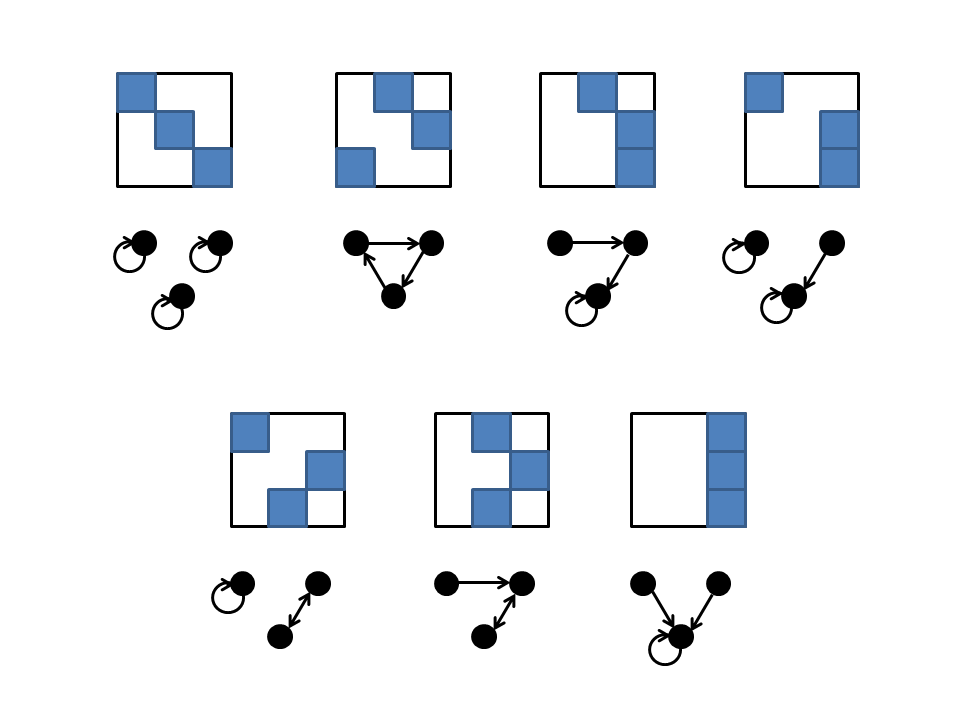
\includegraphics[width=0.6\textwidth]{figures/genpcca.png}
	\caption{Possible structures that can be revealed by GenPCCA.}
	\label{fig:genpcca}
\end{figure}

GenPCCA+ is not only able to identify metastable sets, but also cycles or mixtures of both structures, as depicted in figure \ref{fig:genpcca}. \marginpar{sinks?}
%Why can they be detected?
They can be detected since we consider the dominant eigenvalues and Schur blocks with respect to the absolute value.
Dominant cycles correspond to large eigenvalues $|\lambda| \approx 1$.
\newpage


\subsubsection*{Conclusion}

Even though the Schur decomposition is known for a long time, being described by Schur\cite{schur1909characteristic} in 1909, the approach to utilize it for identifying metastable sets is relatively new. %determine/detect/identify. discovered/described
%classify
There is a huge amount of scientific papers using eigenfunctions or eigenvectors to cluster a process into metastable sets. The entire framework of Markov State Models is built on the spectral analysis of the transfer operator respectively transition matrix; at the beginning in terms of hard sets, nowadays in terms of fuzzy sets.
%Especially it solves one of the main disadvantages of Eigen approach: can handle nonreversible processes!!
%(for reversible: same, nonreversible: only possible on Schur)
Since the Schur decomposition is a generalization of the spectral decomposition, it seems to be an appropriate enhancement of this well-known clustering method.
%first proposed by Röblitz in thesis. Now used from Weber. Weber, Fackeldey .. Djurdevac..
%Still there are very few papers concerning the topic of Schur decomposition to clustering.. in general few papers about nonreversible processes...
%so we see a lot of potential in this approach
%so there is still a lot of potential to develop this theory?
Its main advantages are:
\begin{itemize}
	\item Schur decomposition \textbf{alway}s exists, %can always be constructed to be orthogonal + span inv. subspace
	\item includes reversible as well as \textbf{non-reversible} processes,
	\item orthogonality with respect to \textbf{any} initial distribution $\eta$, %(instead only stationary distribution as for eigenvectors)
	\item detects not only metastable sets, but also \textbf{dominant cycles} and \textbf{sinks}(?), %different structures
	\item Schur decomposition is \textbf{well-conditioned}.
	%In contrast to the eigenvalue problem (bad conditioned \cite[Subsection 7.2.2]{golub1996}),
\end{itemize}
In contrast, the disadvantages are not too dramatic:
\begin{itemize}
	\item Schur decomposition is not unique, \marginpar{?}
	\item Does not exist for a continuous transfer operator.
\end{itemize}

%In addition to metastabilities, dominant cycles and sinks can be identified too
%However/Besides/beyond that
%The main point in employing the Schur decomposition was to extend PCCA+ to non-reversible processes. Beyond that, this approach obviously brings many other advantages along, making this procedure even more flexible (arbitrary $\eta$) and general (detects cycles and sinks as well) than the original PCCA+. %more powerful. ALWAYS appliable!
%,being even more flexible and general than the original PCCA+
%\\

%broader class covered. with the aid of GenPCCA/Schur decomposition
%Additionally, a broader class/set of matrices can be analyzed with the aid of GenPCCA based on the Schur decomposition. This new approach does not only extend PCCA+ to nonreversible processes (huge progress/advance), but also enables us to detect/identify further dominant structures; not only metastable sets but also cyclic structures.
%The main advantage of the Schur decomposition is that we can examine reversible as well as nonreversible processes with it.
The main point in employing the Schur decomposition was to extend PCCA+ to non-reversible processes, which is already a strong improvement.
%However, it brings along many other benefits in comparison to the eigendecomposition.
Beyond that, this approach brings several further advantages along, being more flexible than the original PCCA+ and allowing to identify a broader class of structures.
%yielding a more flexible and general clustering. (arbitrary $\eta$). (detects cycles and sinks as well)
Though, these different structures are not of particular interest in this thesis. %dominant cycles